\documentclass[a4paper]{report}
\usepackage{a4wide}
\usepackage[utf8]{inputenc}
\usepackage{parskip}
\usepackage{hyperref}
\usepackage{epsfig}
\usepackage{background}
\usepackage{mathptmx}

% To avoid tikz error, see https://tex.stackexchange.com/questions/165929/semiverbatim-with-tikz-in-beamer
\makeatletter
\global\let\tikz@ensure@dollar@catcode=\relax
\makeatother

\backgroundsetup{
scale=1,
angle=0,
opacity=1,
contents={
\includegraphics[width=\paperwidth,height=\paperheight]{images/spi-front.jpg}}
}

\hypersetup{
  colorlinks   = true,
  urlcolor     = blue,
  linkcolor    = blue,
  pdfinfo = {
    Title = {SPI Annual Report 2019},
    Author = {Software in the Public Interest, Inc.},
    Keywords = {SPI, free software, open source, FOSS, annual report, charity, non-profit, 501c3},
  }
}

\begin{document}

\title{Software in the Public Interest, Inc.\\
2019 Annual Report}
\date{XXXX XX, 2019}

\maketitle

\newpage

\backgroundsetup{
scale=1,
angle=0,
opacity=1,
contents={
\includegraphics[width=\paperwidth,height=\paperheight]{images/spi-content.jpg}}
}

\hspace{1em}

To the membership, board and friends of Software in the Public Interest, Inc:

As mandated by Article 8 of the SPI Bylaws, I respectfully submit this annual
report on the activities of Software in the Public Interest, Inc. and extend my
thanks to all of those who contributed to the mission of SPI in the past year.

  \emph{-- Michael Schultheiss, SPI President}

\newpage

\tableofcontents

\newpage

\chapter{President's Welcome}
\label{sec:president}

FIXME

  \emph{-- Michael Schultheiss, SPI President}

\chapter{Committee Reports}
\section{Membership Committee}

\subsection{Statistics}

On January 1, 2019 we had 212 contributing and 1082 non-contributing
members.  On December 31, 2019 there were 222 contributing members and
1138 non-contributing members.

\chapter{Board Report}
\section{Board Members}

Board members as of January 1, 2019:

\begin{itemize}
\item Jimmy Kaplowitz (President)
\item Luca Filipozzi (Vice President)
\item Tim Potter (Secretary)
\item Michael Schultheiss (Treasurer)
\item Stephen Frost
\item Dimitri John Ledkov
\item Martin Michlmayr
\item Andrew Tridgell
\item Martin Zobel-Helas
\end{itemize}

Board members as of December 31, 2019:

\begin{itemize}
\item Michael Schultheiss (President)
\item Stephen Frost (Vice President)
\item Tim Potter (Secretary)
\item Martin Zobel-Helas (Treasurer)
\item Luca Filipozzi
\item Forrest Fleming
\item Chris Lamb
\item Héctor Orón Martínez
\item Andrew Tridgell
\end{itemize}

Advisors to the board as of December 31, 2019:

\begin{itemize}
\item Software Freedom Law Center (SFLC), legal counsel
\item Sam Hartman, Debian Project representative
\item Robert Treat, PostgreSQL Project representative
\end{itemize}

\section{Board Changes}

Changes that occurred during the year:

\begin{itemize}

\item Martin Michlmayr resigned from the board in March 2019.
We'd like to thank Martin for his contributions!

\item The board appointed Renee Phillips as an interim director in
April 2019.

\item The terms for Dimitri John Ledkov, Jimmy Kaplowitz, Renee Phillips
and Martin Zobel-Helas expired in July 2019.  Martin sought, and
obtained, re-election.  We'd like to thank Dimitri John Ledkov, Jimmy
Kaplowitz and Renee Phillips for their work on the board.  Forrest
Fleming, Chris Lamb and Héctor Orón Martínez joined the board as part
of the same election.

\item On August 12, 2019 the board voted to appoint the following
officers:

\begin{itemize}
\item President: Michael Schultheiss
\item Vice President: Stephen Frost
\item Secretary: Tim Potter
\item Treasurer: Martin Zobel-Helas
\end{itemize}

\end{itemize}

\section{Elections}

A board membership election was conducted in July 2019.  There were 4
board seats up for election.  Nominations were received from Forrest
Fleming, Chris Lamb, Héctor Orón Martínez and Martin Zobel-Helas.  Since
there were 4 nominations for 4 board seats, no vote was required and all
four candidates were elected for a 3 year term.

\section{Face-to-face Meetings}

The SPI board held two face-to-face meetings in 2019.

At the end of February and the beginning of March, a treasurer sprint
was held for two days, followed by a two-day board meeting.  Meeting
space was kindly provided by the Fintech Open Source Foundation
FINOS) and Crunchy Data.

During the treasurer sprint, the team worked on closing the books
for 2018.  There was also discussion about improving the processes
and workflows and creation more documentation.

During the board meeting, topics such as IT, contractors, budgets
and the intake process were discussed.

The board held another meeting in November 2019 with the newly
elected board.  Meeting space was provided by Hudson River Trading
in New York.  The board discussed the results from the first external
audit, contractors, policies and documentation, infrastructure,
and other topics.  During a proceeding treasurer sprint, outstanding
payment requests were worked on.

\begin{figure*}[h]
\centering

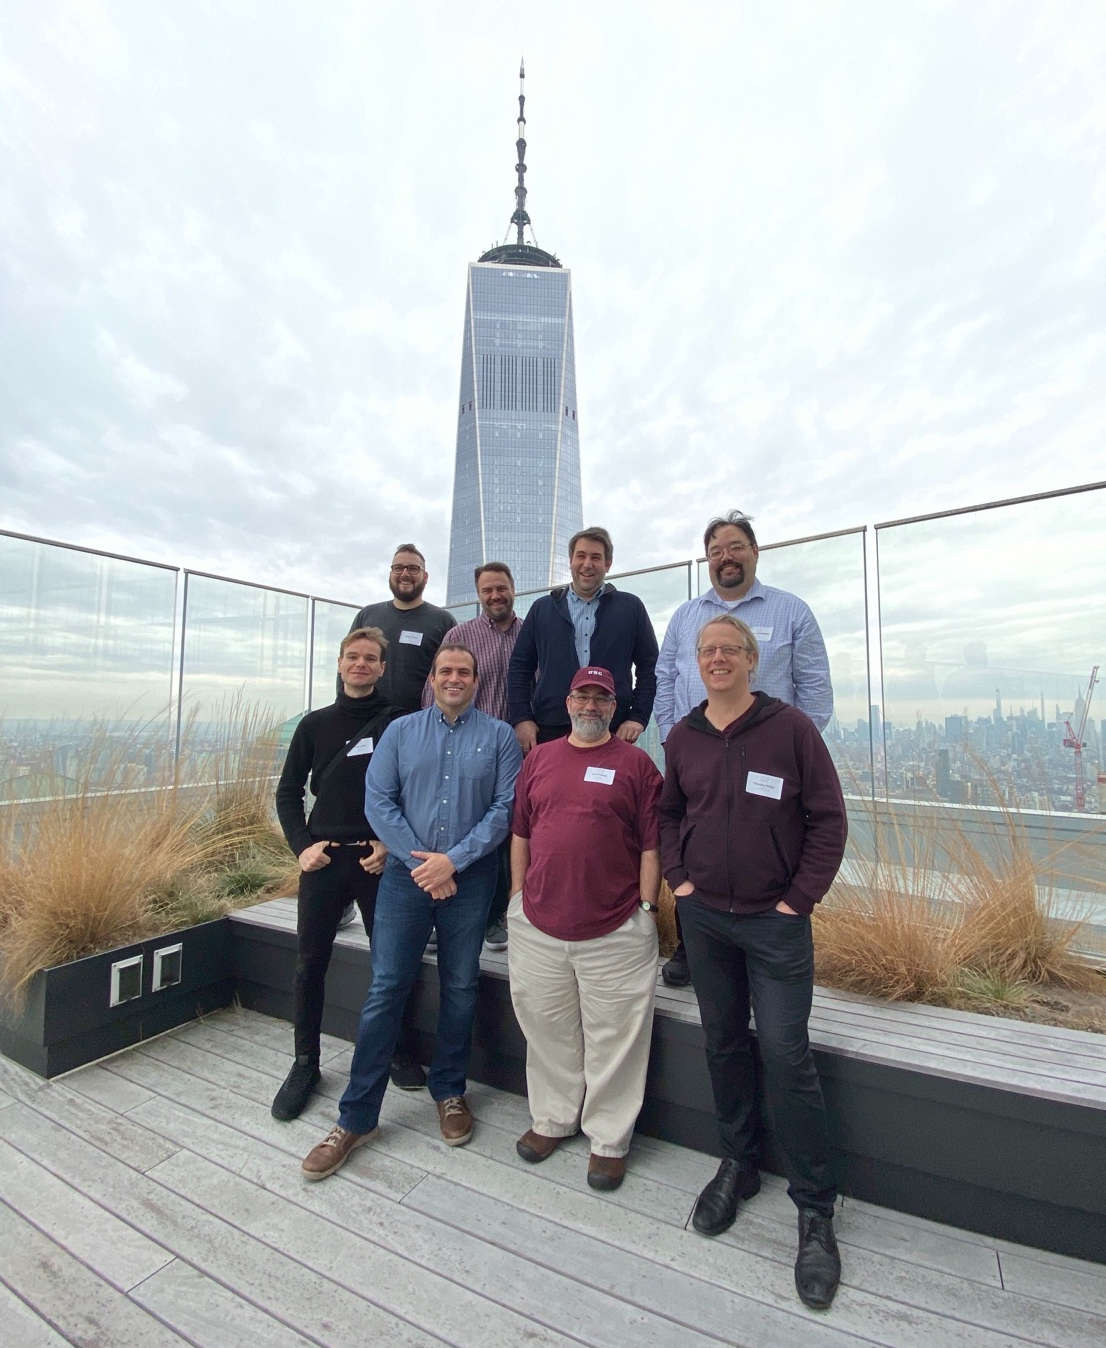
\includegraphics[scale=1.25]{images/2019-november-f2f}

\caption{Face-to-face meeting in New York (November 2019). Front (left
to right): Chris Lamb, Héctor Orón Martínez, Luca Filipozzi, and Tim
Potter.  Back: Forrest Fleming, Stephen Frost, Martin Zobel-Helas,
and Michael Schultheiss}

\end{figure*}

\chapter{Treasury Report}

This report uses a cash-based method of accounting, recording donations
when deposited (not when the check was written or received by us) and
recording expenses when sent or scheduled for payment (not when
incurred).

{\em These figures are provisional and subject to change.}

\section{Income Statement}

This covers the Period January 1, 2019 -- December 31, 2019

\begin{verbatim}
FIXME
\end{verbatim}

\section{Balance Sheet}

\begin{verbatim}
Balance Sheet as of December 31, 2019

FIXME
\end{verbatim}

\chapter{Member Project Reports}

\section{New Associated Projects}

\subsection{Arch Linux 32}

Archlinux32 is a community maintained fork of the Arch Linux
distribution for Intel 32-bit (IA-32) type of CPUs (similar of what
ArchlinuxARM is doing for ARM-based CPUs).

The official support for Intel 32-bit (IA32) has been dropped as of
November 2017.  Archlinux32 plays the catch-up game with upstream Arch
Linux to still provide a usable 32-bit version of Arch Linux.

Archlinux32 has a sophisticated build system keeping track of all
dependencies between packages.  This is especially challenging as
important packages can stop building any time and people expect packages
to be on the bleeding edge (the very purpose of Arch Linux).

\subsection{OpenSAF}

OpenSAF is an open source community with projects focused on high
availability (HA) middleware.  The goal of OpenSAF projects is to
develop HA middleware that is consistent with the Service Availability
Forum (SA Forum) specifications).

\subsection{Translatewiki.net}

Translatewiki.net is a translation community and a localization platform
for free and open source projects. It started out with localization for
MediaWiki. Later support was added for MediaWiki extensions, FreeCol and
other free and open source projects.

\section{Projects No Longer Associated with SPI}

\begin{itemize}

\item Drizzle was fork of the MySQL project originally made in 2008.
The project has been defunct for many years and is no longer under
active development.

\item Freedesktop.org merged its efforts with X.Org, an SPI associated
project.

\item Jenkins is a founding member of the Continuous Delivery Foundation
(CDF) and is in the process of moving its operational functions over to
the CDF.

\item Torch is no longer in active development and has been obsoleted
by PyTorch.  PyTorch is not an associated project of SPI.

\end{itemize}


\appendix
\chapter{About SPI}

SPI is a non-profit organization which was founded to help organizations
develop and distribute open hardware and software. We encourage programmers
to use the GNU General Public License or other licenses that allow free
redistribution and use of software, and hardware developers to distribute
documentation that will allow device drivers to be written for their product.

SPI was incorporated as a non-profit organization on June 16, 1997 in the state
of New York. Since then, it has become an umbrella organization for projects
from the community.

In 1999, the Internal Revenue Service (IRS) of the United States government
determined that under section 501(a) of the Internal Revenue Code SPI
qualifies for 501(c)(3) (non-profit organization) status under section 509(a)(1)
and 170(b)(1)(A)(vi). This means that donations made to SPI and its
supported projects are tax-deductible as charitable donations for US taxpayers.

\newpage

\pagestyle{empty}

\backgroundsetup{
scale=1,
angle=0,
opacity=1,
contents={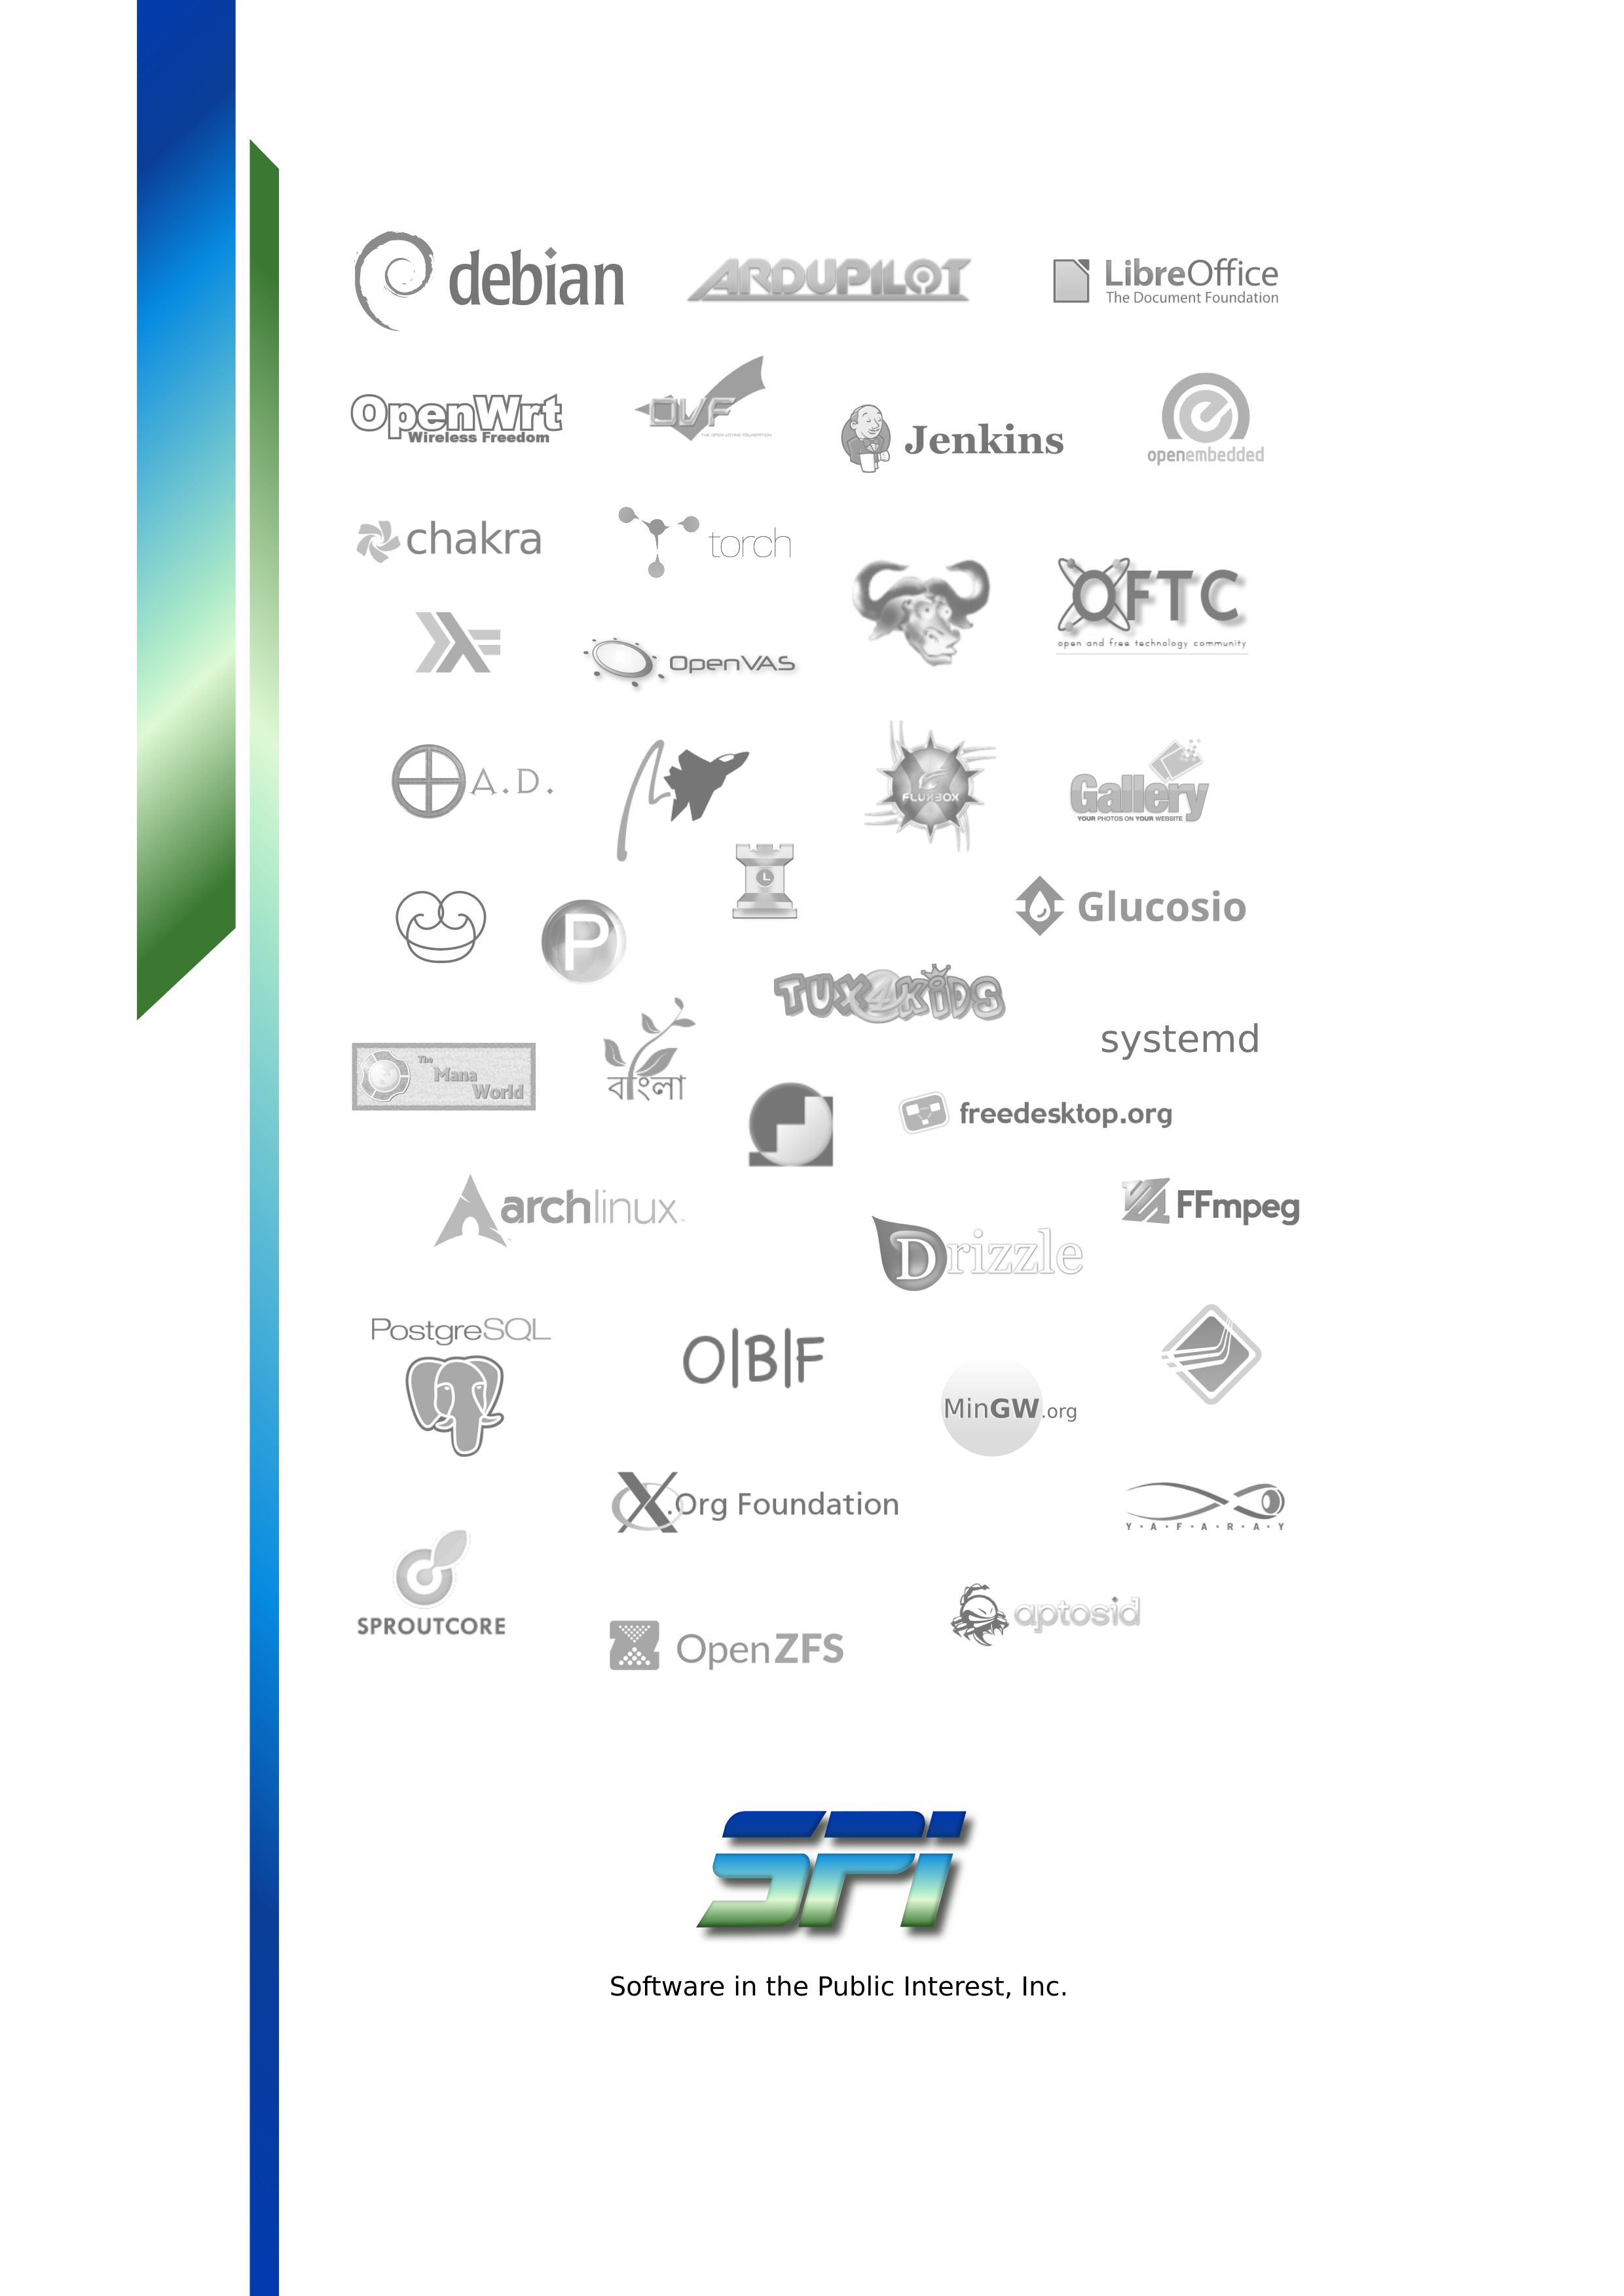
\includegraphics[width=\paperwidth,height=\paperheight]{images/spi-back-2018.jpg}}
}

\null

\end{document}
% Keep this at the bottom, thanks.
% Local Variables:
% TeX-master: "report"
% End:
